\section{Results}
\label{results}

Our Spark program was developed in Scala, run on a machine with two physical CPUs. Each CPU has 16 cores, giving us a total 32 cores. It also houses 32GB of RAM and 1TB of disk space, and runs Ubuntu 16.04. We also used the Hadoop distribution 2.7.2 and the Eclipse IDE configured for spark development. What kind of processor model?

Our graph consisted of 199004 connected components, with the maximum component size at 145 and the minimum at 2. In fact, the distribution of component sizes follow a power law as shown in the following diagram?

For each scenario we vary the number of threads and partitions, compute the percentage of loss, and plot this value against the percentage of nodes removed from the graph. From Fig. \ref{}? we see that...

The run-times and efficiency for each pair of ({\it thread},{\it partition}) values using our input graph are shown in Table \ref{tab:graph1}. How does the number of partitions map to the number of tasks? How to verify it? How does the mapping between partitions and tasks correspond to data locality if any? Reserved threads?

To investigate the effect of increasing input on the scalability of our code, we replicate the graph by doubling it (Table \ref{tab:graph2}) then quadrupling it (Table ref{tab:graph4}). It is evident that our tool offers improved scalability as the input size grows?

%Our own Spark implementation of contingency analysis executes in real-time for the entire power grid, achieving a speed-up of ? on ? processors. We conclude with a spatial understanding of the hotspots on Lebanese soil where energy centers can be exposed and are at risk, using a spatial correlation supported by a binary search tree. The amenability of our work to big data processing makes it extendable to larger networks of networks, towards a fuller understanding of resilence at many vital levels beyond the power grid. Examples are as communications network, Internet networks, transportation networks, hospitals and medical centers networks, to name a few.


\begin{table*}[t]
\begin{minipage}[b]{\textwidth}
\label{tab:threshold-percentage}
\caption{Percentage of vertices to be removed to reach 60\% and 80\% losses}
{\small
\begin{tabular}{||c||c|c|c|c||}
\hline
\textbf{Loss}	&\cellcolor{black!10}BC&	\cellcolor{black!10}C & \cellcolor{black!10} R & \cellcolor{black!10} D \\ \hline \hline
60\% &		11.6\%&	4.3\%	&59.8\%&	7.7\%	 \\ \hline		
80\%	&		27.8\%&	14.6\%	&79.7\%&	29.5\%	 \\ \hline		
\end{tabular}
}
\end{minipage}
\end{table*}




\begin{figure}
\centering
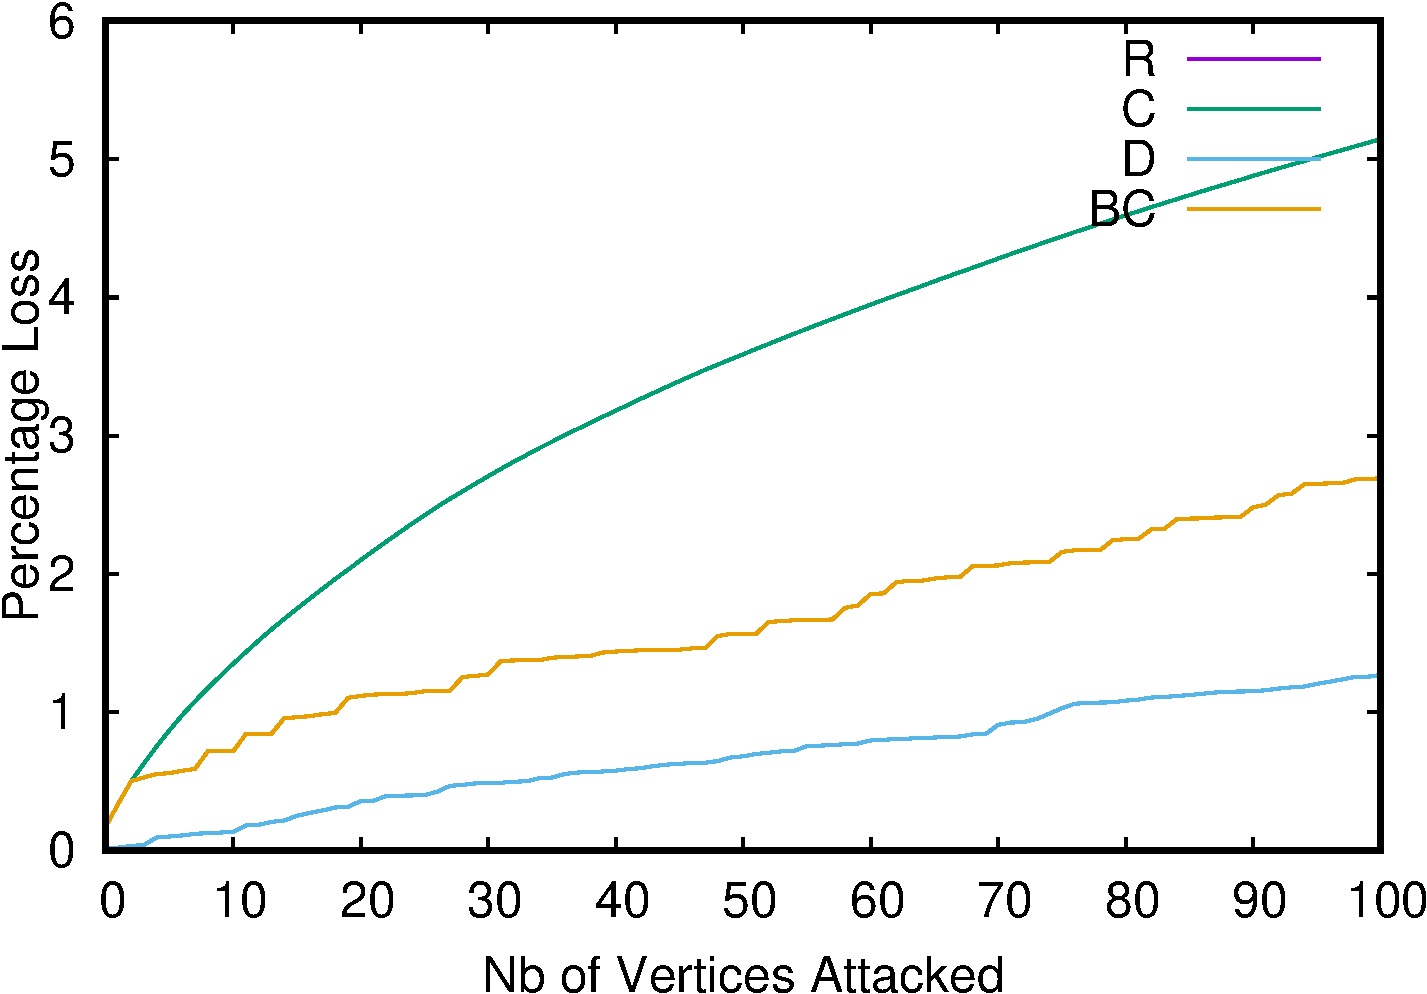
\includegraphics[scale=0.35]{bench/loss-100-crop.pdf}
\label{fig:loss-100}
\caption{Loss percentage: first 100 attacks}
\end{figure}

\begin{figure}
\centering
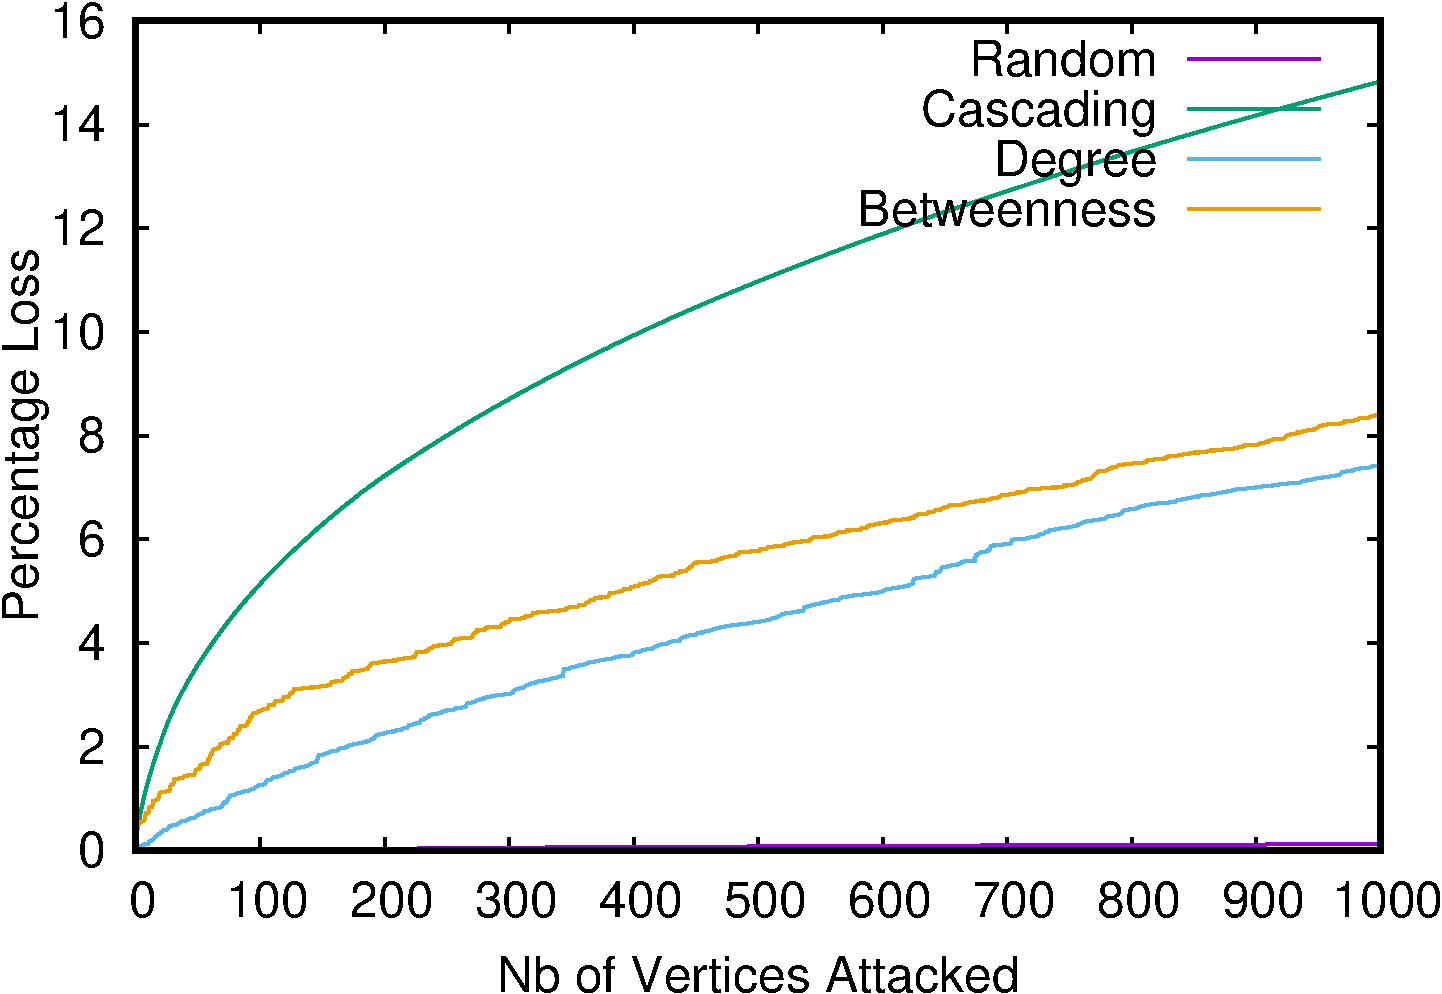
\includegraphics[scale=0.35]{bench/loss-1000-crop.pdf}
\label{fig:loss-1000}
\caption{Loss percentage: first 1000 attacks}
\end{figure}

\begin{figure}
\centering
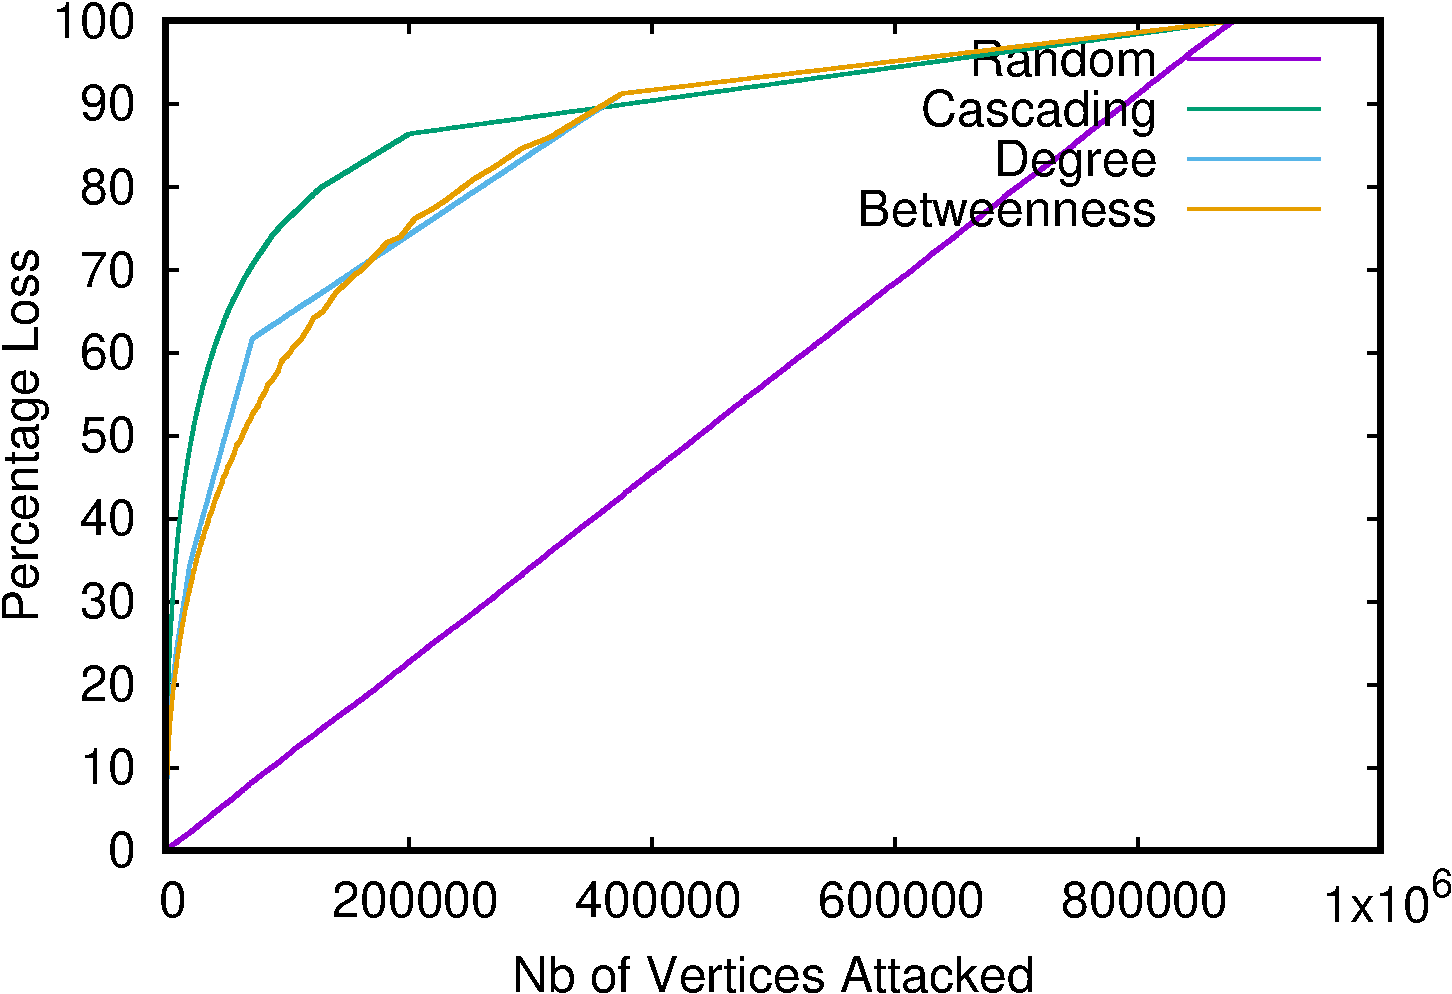
\includegraphics[scale=0.35]{bench/loss-all-crop.pdf}
\label{fig:loss-all}
\caption{Loss percentage: overall attacks}
\end{figure}


\begin{table*}[t]
\begin{minipage}[b]{\textwidth}
\label{tab:graph1}
\caption{Run-times and Efficiency: $\left \vert V \right \vert = 878,969$}
{\small
\centering
\begin{tabular}{||c||c|c|c|c||c|c|c|c||c|c|c|c||c|c|c|c|}
\hline
\textbf{Threads}	&\cellcolor{black!10}BC-4&	\cellcolor{black!10}BC-8	&\cellcolor{black!10}BC-16	&\cellcolor{black!10}BC-32&	\cellcolor{black!10}C-4	&\cellcolor{black!10}C-8&	\cellcolor{black!10}C-16&	\cellcolor{black!10}C-32&	\cellcolor{black!10}D-4&	\cellcolor{black!10}D-8	&\cellcolor{black!10}D-16&\cellcolor{black!10}	D-32&	\cellcolor{black!10}R-4	&\cellcolor{black!10}R-8&	\cellcolor{black!10}R-16&	\cellcolor{black!10}R-32 \\ \hline \hline
64&		27	&17	&22	&41	&53	&34	&32	&52	&26	&15	&20	&41	&23	&17	&20	&39			\\ \hline					
32&		24	&17	&19	&37	&52	&33	&31	&49	&20	&16	&18	&36	&20	&19	&19	&36	\\ \hline
16&		24	&18	&22	&39	&53	&35	&37	&54	&21	&16	&19	&37	&19	&16	&20&37	\\ \hline
8	&	25	&25	&30	&54	&55	&50	&56	&80	&21	&21	&26	&51	&20	&20	&26	&50	\\ \hline
4	&	41	&41	&53	&97	&87	&86	&98	&138	&33	&33	&45	&89	&30	&31	&44	&90	\\ \hline
2&		82	&84	&108	&206	&165	&165	&189	&287	&65	&66	&92	&188	&55	&62	&87	&186	\\ \hline
1&		161	&167	&219	&423	&312	&320	&369	&543	&124	&127	&187	&384	&104	&114	&174	&344	\\ \hline
\end{tabular}
}
\end{minipage}
\end{table*}


\begin{table*}[t]
\begin{minipage}[b]{\textwidth}
\label{tab:graph2}
\caption{Run-times and Efficiency: $\left \vert V \right \vert = 1,757,938$}
{\small
\begin{tabular}{||c||c|c|c|c||c|c|c|c||c|c|c|c||c|c|c|c|}
\hline
\textbf{Threads}	&\cellcolor{black!10}BC-4&	\cellcolor{black!10}BC-8	&\cellcolor{black!10}BC-16	&\cellcolor{black!10}BC-32&	\cellcolor{black!10}C-4	&\cellcolor{black!10}C-8&	\cellcolor{black!10}C-16&	\cellcolor{black!10}C-32&	\cellcolor{black!10}D-4&	\cellcolor{black!10}D-8	&\cellcolor{black!10}D-16&\cellcolor{black!10}	D-32&	\cellcolor{black!10}R-4	&\cellcolor{black!10}R-8&	\cellcolor{black!10}R-16&	\cellcolor{black!10}R-32 \\ \hline \hline
64		&127	&71	&48	&55	&119	&64	&60	&76	&108	&58	&45	&53	&45	&32	&31	&50		 \\ \hline		
32		&120	&59	&45	&49	&116	&68	&56	&71	&108	&57	&42	&47	&40	&29	&29	&45		 \\ \hline			
16		&128	&66	&39	&52	&115	&66	&65	&79	&112	&57	&36	&50	&41	&33	&30	&46 \\ \hline				
8		&123	&66	&56	&77	&120	&97	&98	&121	&106	&54	&46	&68	&40	&34	&39	&63	 \\ \hline			
4		&164	&104	&101	&142	&210	&191	&185	&223	&134	&83	&80	&119	&60	&57	&69	&113	 \\ \hline			
2		&263	&203	&207	&292	&416	&353	&366	&462	&209	&159	&153	&239	&111	&110	&131	&224	 \\ \hline		
1		&452&357	&371	&525	&761	&804	&793	&969	&355	&281	&286	&434	&196	&201	&230	&402 \\ \hline		
\end{tabular}
}
\end{minipage}
\end{table*}


\begin{table*}[t]
\begin{minipage}[b]{\textwidth}
\label{tab:graph4}
\caption{Run-times and Efficiency: $\left \vert V \right \vert = 3,515,876$}
{\small
\begin{tabular}{||c||c|c|c|c||c|c|c|c||c|c|c|c||c|c|c|c|}
\hline
\textbf{Threads}	&\cellcolor{black!10}BC-4&	\cellcolor{black!10}BC-8	&\cellcolor{black!10}BC-16	&\cellcolor{black!10}BC-32&	\cellcolor{black!10}C-4	&\cellcolor{black!10}C-8&	\cellcolor{black!10}C-16&	\cellcolor{black!10}C-32&	\cellcolor{black!10}D-4&	\cellcolor{black!10}D-8	&\cellcolor{black!10}D-16&\cellcolor{black!10}	D-32&	\cellcolor{black!10}R-4	&\cellcolor{black!10}R-8&	\cellcolor{black!10}R-16&	\cellcolor{black!10}R-32 \\ \hline \hline
64 &		525&	317	&171&	117	&411	&179&	127	&123	&430	&220	&134	&104&	133&	79&	70	&87	 \\ \hline		
32	&	491&	274	&153	&99	&387	&202	&123	&121 &449	&243&	149&	100	&122	&101&	64&	75\\ \hline
16	&	473	&311	&133	&96	&401	&184	&127	&137 &457	&236	&113	&77	&130	&86	&62	&78 \\ \hline
8	&	557&	250	&132	&126	&387	&234	&204	&212 &452	&222	&113	&105	&119&	93	&75	&93 \\ \hline
4		&750&	333	&221	&234	&612	&431	&374	&398 &601	&274 &168	&190	&151	&126&	120	&163 \\ \hline
2		&1041 &526 &430 &467	&1042	&791	&736	&793 &888	&436	&344	&395	&273	&235	&237	&337 \\ \hline
1		&1626&902&879 &1021 &2156 &1784 &1577 &1754 &1584 &905 &730 &783& 533 &458 &456 &647 \\ \hline
\end{tabular}
}
\end{minipage}
\end{table*}
